% ICSE 2027 Research Track -- double-anonymous submission, 10 pages main text + 2 pages references.
% The CfP mandates exactly \documentclass[10pt,conference]{IEEEtran};
% no compsoc/compsocconf options, no spacing or font-size alterations.
%
% EVALUATION NUMBERS ARE PLACEHOLDERS. Every number that comes from the experiments is written
% \R{macroName}. The macro is defined by evaluation/analysis/follow_up_aggregate.py in
% ../evaluation/results/follow-up-study/tables/macros.tex; until that file exists (or if a macro is
% missing) \R prints a red "XX". Tables and figures are \input / \includegraphics'ed from the same
% directory and fall back to a placeholder box. Nothing in the text below is a measured result unless
% it is wrapped in \R{...}.
\documentclass[10pt,conference]{IEEEtran}
\IEEEoverridecommandlockouts

% --- Symbols & Custom Marks ---
\usepackage{pifont}
\newcommand{\cmark}{\ding{51}}
\newcommand{\xmark}{\ding{55}}
\newcommand{\pmark}{\ding{109}} % partial coverage

% --- Core Packages ---
\usepackage{cite}
\usepackage{amsmath,amssymb,amsthm,amsfonts}
\usepackage[expansion=false]{microtype}
\usepackage{booktabs, multirow, array}
\usepackage{xcolor}
\usepackage{graphicx}
\usepackage{textcomp}

% --- Visualization ---
\usepackage{tikz}
\usetikzlibrary{arrows.meta,positioning,shapes.geometric,fit,backgrounds,calc}

% --- Algorithms & Code ---
\usepackage{algorithm}
\usepackage[noend]{algpseudocode}
\usepackage{listings}

% --- Layout & Utility ---
\usepackage{enumitem}
\usepackage{hyperref}
\usepackage{cleveref}
% Double-anonymous: keep PDF metadata free of author information.
\hypersetup{hidelinks, pdfauthor={}, pdfsubject={}, pdfkeywords={}}

% --- Theorem environments ---
\theoremstyle{definition}
\newtheorem{definition}{Definition}
\newtheorem{proposition}{Property}

% --- Listing style ---
\lstdefinelanguage{ATL}{
  morekeywords={module,create,from,rule,to,lazy,unique,helper,def,
                context,uses,thisModule,and,or,not,in},
  morekeywords=[2]{@llm,@check}, alsoletter={@},
  sensitive=true, morecomment=[l]{--}, morestring=[b]'}
\lstset{frame=single, backgroundcolor=\color{gray!5},
        basicstyle=\ttfamily\scriptsize, breaklines=true,
        showstringspaces=false, numbers=none, upquote=true,
        keywordstyle=\bfseries, keywordstyle={[2]\bfseries\color{purple}},
        commentstyle=\itshape\color{black!60},
        captionpos=t, abovecaptionskip=2pt, belowcaptionskip=5pt, framesep=2pt,
        aboveskip=6pt, belowskip=4pt, xleftmargin=2pt, xrightmargin=2pt}
\renewcommand{\lstlistingname}{Listing}
% IEEEtran's \@makecaption lets listing frames overlap the caption; use a plain one.
\makeatletter
\def\lst@makecaption#1#2{{\centering\footnotesize #1.\ #2\par}\vspace{4pt}}
\makeatother
\crefname{lstlisting}{Listing}{Listings}
\Crefname{lstlisting}{Listing}{Listings}
\crefname{algorithm}{Algorithm}{Algorithms}
\crefname{proposition}{Property}{Properties}

% --- Math shorthands ---
\newcommand{\tool}{\textsc{AgentM2M}}
\newcommand{\devteam}{\textsc{DevTeam}}
\newcommand{\MM}{\mathit{MM}}
\newcommand{\Mods}[1]{\mathcal{M}(#1)}
\newcommand{\TL}{\mathit{TL}}
\newcommand{\team}{\mathcal{T}}
\newcommand{\cls}[1]{\textsf{#1}}
\newcommand{\code}[1]{\texttt{#1}}
\newcommand{\fp}{\mathit{fp}}
\newcommand{\Obl}{\mathit{Obl}}
\newcommand{\dig}{\mathrm{dg}}
\newcommand{\sel}{\mathit{sel}}
\newcommand{\Ctx}{\mathcal{C}}
\newcommand{\Infl}{\mathit{Infl}}
\newcommand{\pol}[1]{\textsf{#1}} % knowledge-distribution policy name
\DeclareRobustCommand{\tracemark}{\tikz[baseline=-0.6ex]\node[draw,diamond,fill=black!70,inner sep=1.1pt]{};}

% --- Evaluation placeholders (see header) ---
\newcommand{\RESDIR}{../evaluation/results/follow-up-study}
\IfFileExists{\RESDIR/tables/macros.tex}{\input{\RESDIR/tables/macros.tex}}{}
\newcommand{\R}[1]{\ifcsname #1\endcsname\csname #1\endcsname\else\textcolor{red}{\textbf{XX}}\fi}
% \resulttable{name}{width-fallback-tabular}: the generated tabular, scaled to the column.
\newcommand{\resulttable}[2]{%
  \IfFileExists{\RESDIR/tables/#1.tex}{\resizebox{\columnwidth}{!}{\input{\RESDIR/tables/#1.tex}}}{\resizebox{\columnwidth}{!}{#2}}}
\newcommand{\resultfigure}[2]{%
  \IfFileExists{\RESDIR/figures/#1.pdf}{\includegraphics[width=#2\linewidth]{\RESDIR/figures/#1.pdf}}{%
    \fbox{\parbox{#2\linewidth}{\centering\vspace{14mm}\textcolor{red}{\textbf{[figure \texttt{\detokenize{#1}} -- placeholder]}}\vspace{14mm}}}}}
\newcommand{\XX}{\textcolor{red}{\textbf{XX}}}

\begin{document}

\title{Selective Knowledge Pinning for LLM Agent Teams:\\
Traceable, Observable, and Cheaper Shared Context}

% --- Double-anonymous review: no author block in the submission. ---
% \author{...}

\maketitle

\begin{abstract}
LLM agent teams share more than artifacts: a finding, a design decision, or a constraint must reach
the agents that depend on it, and when it changes, the work derived from it must be redone. In
practice this knowledge is pasted into prompts, so nothing records which decision used which
version, a change either re-runs everything or relies on someone's routing table, and the
collaboration cannot be observed without reading transcripts. We extend a transformation-based
agent runtime, whose LLM calls are bounded by declared footprints and version stamps, with three
mechanisms for \emph{knowledge}. (1) A versioned, access-controlled \emph{shared context} whose
\emph{selected} items are pinned into each binding's stamp, and which fails closed when a declared item
cannot be resolved. (2) An \emph{influence query} over the recorded pins. (3) An \emph{observability
plane}: a typed event timeline, optionally projected to Nostr relays as signed events, designed not to
influence the run. We state the properties
the design gives and the assumptions they need, and test them on \R{ctxRepos} DevBench
repositories with \R{ctxModels} open-weight model(s) in \R{ctxRuns} runs of a five-revision schedule
against four distribution policies: naive paste, hand-routed paste, whole-context pinning, and
item-level pinning. Item-level pinning delivered revised knowledge to \R{rqOneCtxiDeliveredNew} of
the artifacts that had to change (routed paste: \R{rqOneRoutedDeliveredNew}), at
\R{rqTwoRatioCtxiVsPaste}$\times$ fewer tokens than naive paste and \R{rqTwoRatioCtxiVsRouted}$\times$
the cost of routed paste, which a team must maintain by hand. Attaching Nostr left state and prompts
identical in \R{obsNostrStateIdentical} of replays, and \R{faultDetectedShare} of \R{faultTested}
injected faults were surfaced; two probes of what the design cannot see stayed silent, as expected.
\end{abstract}

\begin{IEEEkeywords}
LLM-based multi-agent systems, shared context, traceability, observability, model transformation,
incremental computation, software engineering agents
\end{IEEEkeywords}

\section{Introduction}\label{sec:introduction}

Teams of LLM agents now analyze, design, implement, and test software together. Role-based frameworks
assign an analyst, a coder, and a tester to separate model instances~\cite{dong2024selfcollab}. Others
encode standard operating procedures as hand-offs between roles~\cite{hong2024metagpt,qian2024chatdev}, or
coordinate agents around repository issues~\cite{tao2024magis}. He et al.\ review this landscape in TOSEM
and list, among its open problems, how agents share what they know and how their collaboration is
organized~\cite{he2025lma}. The failure data point the same way. Cemri et al.\ identify
\emph{inter-agent misalignment}, where an agent withholds information, ignores another agent's input, or
acts on a stale view of it, as one of three failure categories of multi-agent LLM
systems~\cite{cemri2025mast}.

\smallskip\noindent\textbf{What a team transfers.} Software engineering has studied knowledge transfer
in \emph{human} teams for two decades, and we use those studies as an organizing frame for agent teams;
we do not claim a complete taxonomy. Ko et al.\ observed 17 developers. They most often sought awareness
about artifacts and coworkers, and the questions they most often had to defer concerned design and intended
behavior, whose only source was an unavailable colleague~\cite{ko2007information}. De Souza and Redmiles
describe how developers work to find out who depends on a change and whose changes affect
them~\cite{desouza2008dependencies}. Cataldo and Herbsleb associate coordination requirements that a team
leaves unmet with lower productivity and more failures~\cite{cataldo2013coordination}. Herbsleb and Mockus
find that work items spanning sites take about two and a half times as long as co-located ones, and trace
the delay to the larger number of people involved and to weaker cross-site
communication~\cite{herbsleb2003speed}. From these studies we take four kinds of knowledge that a team
transfers (\Cref{tab:kt}). \textbf{KT1} is the content of \emph{artifacts} passed between stages.
\textbf{KT2} is \emph{cross-cutting knowledge} that is not an artifact of any stage: a design decision, a
constraint, a review finding. \textbf{KT3} is knowledge of \emph{change and dependency}: what changed, and
who must react. \textbf{KT4} is \emph{awareness}: who did what, and who knows what~\cite{mockus2002expertise}.
Questions about runtime behavior, such as the cause of a program state~\cite{ko2007information}, fall
outside this frame.

\begin{table}[t]
\centering
\caption{Organizing frame: knowledge a team transfers, what human-team studies observed, the channel LLM
agent teams use today, and the issue that channel raises.}
\label{tab:kt}
\scriptsize
\setlength{\tabcolsep}{2.5pt}
\begin{tabular}{@{}>{\raggedright}p{13mm}>{\raggedright}p{21mm}>{\raggedright}p{21mm}>{\raggedright\arraybackslash}p{25mm}@{}}
\toprule
Kind & Human teams & Channel in LLM teams & Issue \\
\midrule
KT1 artifact content & passed between stages & role hand-off, SOP
  documents~\cite{dong2024selfcollab,hong2024metagpt,qian2024chatdev} & \textbf{I1} loss and distortion in
  transfer~\cite{cemri2025mast} \\
KT2 cross-cutting knowledge & design knowledge most often deferred~\cite{ko2007information} & text pasted into
  prompts or context files~\cite{liang2025prompts}; experience pools~\cite{qian2024colearning} &
  \textbf{I2} influence is untraceable \\
KT3 change and dependency & unmet coordination needs associated with failures~\cite{cataldo2013coordination} &
  re-run everything, or a planner~\cite{bairi2024codeplan} & \textbf{I3} stale knowledge;
  \textbf{I4} redundant regeneration \\
KT4 awareness & most often sought~\cite{ko2007information}; distance delays work~\cite{herbsleb2003speed} &
  transcripts and trajectories~\cite{bouzenia2025trajectories,dong2024agentops} & \textbf{I5} opaque
  collaboration \\
\bottomrule
\end{tabular}
\end{table}

\smallskip\noindent\textbf{Issues raised in LLM agent teams.} \textbf{I1}: in a transfer, content is lost
or distorted, which is the inter-agent misalignment of Cemri et al.~\cite{cemri2025mast}. Missing knowledge
also hurts a single agent: Zhang et al.\ trace part of the hallucinations in repository-level code
generation to conflicts with project context the model was not given~\cite{zhang2025hallucination}.
\textbf{I2}: once knowledge is pasted into a prompt, nothing records which decision used which version of
it. Liang et al.\ argue from interviews that prompts are programs and call for program-like
tooling~\cite{liang2025prompts}. Even links that humans must record by hand are often missing: Rath et al.\
found only about 60\% of commits in six open-source projects linked to an issue~\cite{rath2018traceability}.
\textbf{I3}: when knowledge changes, the work derived from it goes stale unless someone knows what depends on
it, the coordination problem of human teams~\cite{desouza2008dependencies,cataldo2013coordination}. For code,
CodePlan needs dependency and change may-impact analysis to propagate one edit through a
repository~\cite{bairi2024codeplan}. \textbf{I4}: to avoid I3, a team re-runs more than it must, and every
repeated call re-reads its context. Token limits are among the challenges LLM application developers
report~\cite{chen2025llmdevchallenges}, long inputs are used less reliably~\cite{liu2024lost}, and cost now
counts alongside effectiveness in evaluations of SE agents~\cite{xia2025agentless}. \textbf{I5}: agents
leave transcripts, and explaining why an agent run succeeds or fails still takes manual trajectory
analysis~\cite{bouzenia2025trajectories}. Protocols such as MCP and A2A standardize how messages
travel~\cite{mcp2024,a2a2025,ehtesham2025interop}, but they do not record which \emph{knowledge version} an
agent used. We know of no study that measures I3 or I4 in agent teams; they follow from the channel, and
RQ1 and RQ2 below provide data on them.

\smallskip\noindent\textbf{Gap.} Current frameworks pass knowledge as messages. MetaGPT, for instance, lets
roles subscribe to a shared message pool~\cite{hong2024metagpt}, and conversational frameworks pass it in
dialogue~\cite{wu2024autogen,qian2024chatdev}. They do not record which version of a shared item a generated
value was conditioned on, and they do not decide which values a change to that item invalidates. Earlier work
on the runtime we extend addresses KT1. There, each hand-off is a model-to-model (M2M) transformation: a
deterministic engine owns structure, trace links, and obligations, and the LLM fills attribute values only
through validated \emph{stochastic bindings} that read a declared source footprint~\cite{anon2027agentm2m}.
KT2--KT4 knowledge stays outside that engine. A security reviewer's finding that \code{download()} must not
write outside its target directory is not an element of any view, so the engine cannot tell which values
used it (I2), which must be redone when it changes (I3, I4), or who used it (I5).

\smallskip\noindent\textbf{Approach.} We add a collaboration plane beside the transformation plane. Knowledge
becomes typed, versioned, attributed \emph{context items} under an access policy. A binding declares, in its
rule, which items it reads, and the digest of exactly those items joins its version stamp. The invalidation
rule is deliberately the standard one of build systems, a hash of a declared read set~\cite{mokhov2018build}.
What is new is what it is applied to and what comes with it. The input is knowledge that is not an artifact;
it is access-controlled and resolved for the agent that owns the target view; and it fails closed when it
cannot be resolved. The leaves are stochastic, so a stamp caches \emph{a} sample, not \emph{the} value. Each
obligation records whether its cause was the source or the context. The \emph{pins} recorded at acceptance
make it a query to find every value generated with an item in its prompt; we call this set the item's
\emph{influence}, meaning exposure, not causal effect (I2). Every transition is emitted as a typed event
through one choke point. The timeline can be projected to Nostr relays as events signed with each agent's own
key, so a run that spans machines can be attributed without a trusted central server (I5). Compared with the
earlier runtime, the delta is the context store, item selection in the stamp, cause recording, pins and the
influence query, the event plane, and relay sync. The declaration of which items a binding reads is still
written by hand. The gain over a hand-kept routing table is that the declaration sits next to its consumer,
the engine enforces it, and its use is recorded. Three limits matter. The design cannot see knowledge pasted
into a prompt literal. It does not judge whether knowledge is right. And it addresses I1 only by giving the
model labelled, attributed items in place of free text. We test the first two limits.

\smallskip\noindent\textbf{Research questions.}
\textbf{RQ1 (delivery and traceability):} when shared knowledge is revised, does the revised knowledge reach
the artifacts that depend on it, and does the recorded influence match what the agents were shown?
\textbf{RQ2 (cost):} what does item-level pinning cost against naive paste, hand-routed paste, and
whole-context pinning, and does it preserve the retention of stated constants?
\textbf{RQ3 (invariants and failure surfacing):} does attaching the observability plane leave the run
unchanged, how completely do events reconstruct it, what does it cost, and which injected failures are
surfaced and which are not?

\smallskip\noindent\textbf{Contributions.}
\textbf{(C1)} Shared knowledge as versioned, access-controlled context whose \emph{selected item digest}
joins the binding stamp. It is specified in five algorithms over the running example of
Section~\ref{sec:background}, with three properties (selective invalidation, fail-closed resolution,
non-interference), each stated with its assumptions and the cases it does not cover
(Section~\ref{sec:approach}).
\textbf{(C2)} An influence query over pinned trace links, and an observability plane with a privacy-tiered
event schema and a signed Nostr projection whose receiver checks seven conditions before it applies a context
version.
\textbf{(C3)} An empirical study on \R{ctxRepos} DevBench repositories that compares item-level pinning with
naive paste, hand-routed paste, and whole-context pinning, tests non-interference by replay, and injects 21
faults, including two probes of what the design cannot detect (Sections~\ref{sec:design}--\ref{sec:results}).
The harness, the logs, the reference-validity script, the script behind every number of the running example,
and the script that generates every number of the study are released (Section~\ref{sec:data}).

\section{Background and Running Example}\label{sec:background}

We introduce the runtime we extend on one running example, which every algorithm of
Section~\ref{sec:approach} uses again. A released script runs the example with a scripted LLM and reproduces
every count quoted in Sections~\ref{sec:background} and~\ref{sec:approach}.

\subsection{Running example: the \code{chakin} team}\label{sec:running}

\code{chakin} is a DevBench repository~\cite{li2024devbench}: a Python library that downloads pre-trained
word vectors. Its UML class diagram has three public functions, \code{load\_datasets()},
\code{download(number, name, save\_dir)}, and \code{search(lang)}, and one test method,
\code{test\_download\_by\_name}, which the team treats as an operation like the others. The study adds five
\emph{canary} operations. Each canary's requirement states a constant, for example a threshold, that the
generated code must keep; canaries measure whether hand-offs preserve stated facts. That makes nine
operations. The team has five agents (\Cref{fig:running}). The \emph{Analyst} owns view $M_{req}$, with one
user story and one acceptance criterion per operation, for example \code{download.C1}. The \emph{Architect}
owns $M_{arch}$, with one \cls{Operation} per story. The \emph{Developer} owns $M_{code}$, with one
\cls{CodeEdit} per operation whose \code{body} is a function. The \emph{Tester} owns $M_{test}$, with one
\cls{TestCase} per criterion whose \code{oracle} is a test function. The \emph{Security Reviewer} owns
$M_{sec}$, with one \cls{Review} per operation, and is added after the first run. Four hand-offs connect the
views: $T_1$ \code{Req2Arch}, $T_2$ \code{Arch2Code}, $T_3$ \code{Req2Test}, which derives tests from the
requirements rather than from the design, and $T_4$ \code{Arch2Sec}.

\begin{figure}[t]
\centering
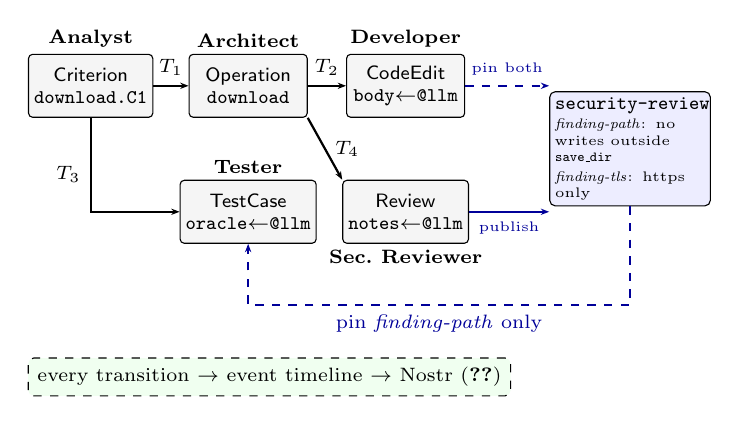
\begin{tikzpicture}[
  font=\scriptsize, >={Stealth[length=3pt]},
  el/.style={draw, rounded corners=1.5pt, fill=gray!8, align=center, inner sep=2pt, minimum width=15mm, minimum height=8mm},
  ag/.style={font=\scriptsize\bfseries, inner sep=1pt},
  ho/.style={->, thick},
  pin/.style={->, thick, blue!60!black, dashed}]
  \node[el] (crit) at (0,0)    {\cls{Criterion}\\\code{download.C1}};
  \node[el] (op)   at (2.0,0) {\cls{Operation}\\\code{download}};
  \node[el] (ce)   at (4.0,0)  {\cls{CodeEdit}\\\code{body}$\leftarrow$\code{@llm}};
  \node[el] (tc)   at (2.0,-1.6) {\cls{TestCase}\\\code{oracle}$\leftarrow$\code{@llm}};
  \node[el] (rv)   at (4.0,-1.6)  {\cls{Review}\\\code{notes}$\leftarrow$\code{@llm}};
  \node[ag, above=1pt of crit] {Analyst};
  \node[ag, above=1pt of op] {Architect};
  \node[ag, above=1pt of ce] {Developer};
  \node[ag, above=1pt of tc] {Tester};
  \node[ag, below=1pt of rv] {Sec.\ Reviewer};
  \draw[ho] (crit) -- node[above]{$T_1$} (op);
  \draw[ho] (op) -- node[above]{$T_2$} (ce);
  \draw[ho] (crit.south) |- node[pos=0.3,left]{$T_3$} (tc.west);
  \draw[ho] (op.south east) -- node[pos=0.5,right]{$T_4$} (rv.north west);
  \node[draw, fill=blue!7, rounded corners=2pt, align=left, text width=19mm, inner sep=2pt, font=\tiny]
       (ctx) at (6.85,-0.8) {\code{\scriptsize security-review}\\[1pt]
       \emph{finding-path}: no writes outside \code{save\_dir}\\[1pt]
       \emph{finding-tls}: https only};
  \draw[->, thick, blue!60!black] (rv.east) -- node[below, font=\tiny]{publish} (rv.east -| ctx.west);
  \draw[pin] (ce.east) -- node[above, font=\tiny]{pin both} (ce.east -| ctx.west);
  \draw[pin] (ctx.south) |- ++(0,-1.25) -| node[pos=0.25, below]{pin \emph{finding-path} only} (tc.south);
  \node[draw, dashed, fill=green!6, rounded corners=2pt, font=\scriptsize, anchor=north west]
       at (-0.8,-3.45) {every transition $\to$ event timeline $\to$ Nostr (\cref{sec:obs})};
\end{tikzpicture}
\caption{Running example on DevBench \code{chakin}, shown for \code{download}. Solid arrows: hand-offs, the
transformation plane (Section~\ref{sec:background}). Blue: the collaboration plane, a shared context and its
pins (Section~\ref{sec:approach}). Green: the observability plane.}
\label{fig:running}
\end{figure}

\subsection{Hand-offs as transformations}\label{sec:handoffs}

\begin{definition}[Team, hand-off, trace link]\label{def:team}
A team is a megamodel, a model whose elements are models and the transformations between them:
$\team=(A,V,\mathbf{T},\omega,\varphi)$ with agents $A$, view metamodels $V$, hand-off transformations
$\mathbf{T}$, write rights $\omega: V\to A$ (one owner per view), and an acceptance predicate
$\varphi$~\cite{anon2027agentm2m}. A hand-off $T_{ij}$ is a set of ATL-style rules~\cite{jouault2008atl} that
read $M_i$ and write $M_j$. A rule $r$ has a source pattern $p_r$, a guard $g_r$, and target bindings. For each
match $m$ it creates a target $t$ and records a persistent trace link $(m,t,r)$ in the trace model
$\TL$~\cite{jouault2005traceability,vara2014metagem}. We write $\omega(t)$ for the owner of $t$'s view.
\end{definition}

Target bindings come in two kinds. A \emph{structural} binding is an OCL-like expression the engine evaluates,
such as \code{name <- op.name}. A \emph{stochastic} binding \code{f <- @llm(prompt, e)} delegates to the LLM
a value that no expression can compute. \Cref{lst:a2c} shows $T_2$. Its footprint \code{op.codeContext()} is
the operation's signature and its specification, which $T_1$ copies structurally from the criterion.

\begin{lstlisting}[language=ATL, float=t, caption={Hand-off $T_2$ (Architect $\to$ Developer) of the
running example, abridged.}, label={lst:a2c}]
rule Operation2CodeEdit {
  from op : Arch!Operation
  to  ce : Code!CodeEdit (
    name      <- op.name,         -- structural
    operation <- op,              -- structural
    body      <- @llm('Implement this operation ...',
                   op.codeContext()), -- stochastic
    @check body.compiles()
       and body.definesName(op.name) ) }
\end{lstlisting}

\begin{definition}[Footprint, stamp, obligation]\label{def:stamp}
The expression $e$ of a stochastic binding $b$ defines its \emph{footprint} $\fp_b(m)$, the only source
values the LLM may see. Let $H$ be SHA-256 truncated to 16 hexadecimal digits (64 bits), computed over a
canonical encoding of the footprint's attribute values. When a value is accepted, the trace link stores the
stamp $\mathit{stamp}(t,b)=H(\fp_b(m))$. The pair $(t,b)$ is an \emph{obligation} iff a stamp exists and
differs from $H$ of the current footprint, and \emph{new} iff no stamp exists. The predicate $\varphi$ holds
iff every match is covered, no obligation or escalation is open, and all stamps are fresh.
\end{definition}

\begin{algorithm}[t]
\caption{Executing a hand-off~\cite{anon2027agentm2m}}
\label{alg:handoff}
\small
\begin{algorithmic}[1]
\Function{HandOff}{$T_{ij}, M_i, M_j, \TL$}
  \State match $M_i$; create, link, or delete targets; evaluate structural bindings \Comment{structure}
  \For{$(m,t,r)\in\TL$, stochastic $b$ of $r$}
    \State $d\gets H(\fp_b(m))$
    \If{$\mathit{stamp}(t,b)=d$} \textbf{continue} \Comment{fresh: no call}
    \EndIf
    \If{$\mathit{failed}(t,b)=d$} report escalation; \textbf{continue}
    \EndIf
    \State $\pi_0\gets \mathit{prompt}_b\oplus\mathit{render}(\fp_b(m))$;\ $\pi\gets\pi_0$
    \For{$a=1..k$}
      \State $v\sim\mathrm{LLM}(\pi)$
      \If{$\mathit{chk}_b(v)$} $t.f_b\gets v$;\ $\mathit{stamp}(t,b)\gets d$;\ \Return
      \EndIf
      \State $\pi\gets\pi_0\oplus\mathit{feedback}(v)$ \Comment{retry with the rejection}
    \EndFor
    \State $\mathit{failed}(t,b)\gets d$ if a sample was rejected; escalate
  \EndFor
\EndFunction
\end{algorithmic}
\end{algorithm}

\Cref{alg:handoff} executes one hand-off. Line~2 owns all structure. Lines~3--12 call the LLM only for
bindings whose footprint digest differs from their stamp, at most $k$ times, and each sample must pass the
binding's validator $\mathit{chk}_b$ (the \code{@check} clause). A binding that exhausts its budget is
\emph{escalated}: it is reported to the team as an open problem, and $\mathit{failed}(t,b)$ remembers the
footprint so that the same prompt is not retried until the footprint changes. Transport failures are not
remembered. The runtime has two modes. In \emph{engine mode} it calls an LLM backend itself. In \emph{host
mode} it hands each pending prompt to an external agent, such as a coding assistant, and judges the value
that agent submits. \Cref{alg:handoff} is incremental computation~\cite{mokhov2018build,hammer2014adapton}
with a stochastic function at the leaves.

\emph{Example.} After the first run all nine \code{body} bindings are stamped. Suppose the Analyst edits
criterion \code{download.C1}. $T_1$ copies the new text into the specification of \code{download}, so
$\fp_{\mathit{body}}(\code{download})$ changes, as do the footprints of the Architect's \code{signature} and
of the Tester's \code{oracle} for \code{download.C1}. Exactly these three bindings are obliged, and three LLM
calls are made; the eight other bodies stay fresh. KT1 transfer is thus already traceable and selective.

\subsection{Knowledge that is not an artifact}\label{sec:problem}

Now the Security Reviewer reads \code{download} and publishes two findings (\Cref{fig:running}).
\emph{finding-path}: \code{save\_dir} comes from the caller, so the function must refuse to write outside it.
\emph{finding-tls}: vectors must be fetched over https only. Both are KT2 knowledge. Neither is an element of
$M_{arch}$, so neither enters $\fp_{\mathit{body}}$, and \Cref{alg:handoff} cannot see them. Today a team
distributes such findings in one of two ways.

\textbf{Naive paste} (\pol{paste}). The text of every finding is pasted into every consumer's prompt. The
prompt literal is not part of the footprint, so a revision creates no obligation. The operator, who has no
record of dependencies, must re-run every consumer (I4) or risk stale code (I3). Nothing records which body
was generated under which version of \emph{finding-path} (I2).

\textbf{Routed paste} (\pol{routed}). Each finding is pasted only into the prompts that need it, and only
those are re-run. Its cost is minimal, but its routing table (``\emph{finding-tls} goes to the Developer
only'') is a dependency graph that an operator keeps and applies by hand. Unmet coordination needs of this
kind are associated with failures in human teams~\cite{cataldo2013coordination}.

\begin{table}[t]
\centering
\caption{Bindings re-run per change in the running example (9 bodies, 9 oracles). \emph{Declared}: consumers
under the pins of \Cref{fig:running}. \emph{Semantic}: bindings whose value the finding is about. \pol{paste}
re-runs on any change of text; \pol{ctx} pins the whole context, \pol{ctxi} the items of \Cref{fig:running}.}
\label{tab:example}
\footnotesize
\setlength{\tabcolsep}{2.6pt}
\begin{tabular}{@{}lrrrrrr@{}}
\toprule
Change & Semantic & Declared & \pol{paste} & \pol{routed} & \pol{ctx} & \pol{ctxi} \\
\midrule
S1 revise \emph{finding-path} & 2 & 18 & 18 & 18 & 18 & 18 \\
S2 revise \emph{finding-tls}  & 1 & 9  & 18 & 9  & 18 & 9 \\
S3 add unrelated note         & 0 & 0  & 18 & 0  & 18 & 0 \\
S4 identical rewrite          & 0 & 0  & 0  & 0  & 0  & 0 \\
\midrule
\multicolumn{3}{@{}l}{Routing declared where?} & -- & table & rule & rule \\
\multicolumn{3}{@{}l}{Routing enforced and recorded?} & no & no & yes & yes \\
\bottomrule
\end{tabular}
\end{table}

\Cref{tab:example} states the problem on the example. \pol{routed} matches the declared set only while its
table is right and is applied. \pol{paste} re-runs everything. Neither records influence. The approach should
re-run what the declarations require, enforce and record them, keep a missing or revoked finding from being
silently replaced, and make all of it observable without changing the run. The table also shows two limits.
Both findings concern \code{download}, which is two bindings (\emph{Semantic}), yet all nine bodies consume
them, because a declaration is per binding, not per match. And no mechanism here can tell whether
\emph{finding-path} is correct. In the study (Section~\ref{sec:design}) the findings are synthetic markers,
so that whether knowledge reached an artifact is decidable; S1 and S2 correspond to its revisions R1, R2, and
R5, S3 to R3, and S4 to R4.

\textbf{Why not shared memory, retrieval, subscription, or prompt versioning?} A blackboard or memory
store~\cite{nii1986blackboard,packer2023memgpt} shares knowledge but does not say which outputs used which
version. Retrieval-augmented generation selects knowledge per call without a declaration, but the selection
then depends on the retriever, so a stamp over it would not be stable. Subscription to a message
pool~\cite{hong2024metagpt} declares interest, but delivery does not invalidate values generated earlier.
Versioning prompts records which prompt version ran, but not which output was derived from which knowledge
version, and it obliges nothing. The approach combines a declared read set, invalidation per binding, and a
record per accepted value.

\section{Approach: Shared Context as a Collaboration Plane}\label{sec:approach}

\Cref{fig:running} shows the three planes, and \Cref{tab:guarantees}, at the end of this section, maps each
issue to its mechanism, its property, and what is not covered. Four design goals follow from
Section~\ref{sec:problem}. \textbf{D1} (enforced declaration): the dependency is declared at the consumer and
enforced by the engine, not decided by an operator at each change. \textbf{D2} (fail closed): a binding whose
declared knowledge cannot be resolved is never answered with empty or invented knowledge. \textbf{D3}
(non-interference): observing a run must not change it. \textbf{D4} (authority): only authorized agents read
or write knowledge, and every item names its real author.

\subsection{Context model and store}\label{sec:store}

\begin{definition}[Item, snapshot, policy]\label{def:context}
A \emph{context item} is a record $i=(\mathit{id},\mathit{type},\mathit{content},\mathit{author},
\mathit{provenance})$. A \emph{context} $c$ is a sequence of immutable \emph{snapshots}
$\sigma_1,\sigma_2,\dots$, each a set of items. For a set of items $S$,
$\dig(S)=\mathrm{SHA256}$ of the canonical records of $S$ sorted by id. For a list of ids $I$, $\sigma|_I$
selects those items, and $\sigma|_{*}$ is all of them. A \emph{policy} $\pi_c=(\mathit{owner},W,R,
\mathit{vis},\mathit{expiry})$ names writers $W$, readers $R$, a visibility ($\mathit{private}$: only listed
agents read; $\mathit{team}$: every agent reads; $\mathit{relay}$: also synchronized across machines), and an
optional expiry.
\end{definition}

The digest covers the whole record and no timestamp. Identical items give an identical digest at any time.
A change of authorship is a change, so re-attributing an item obliges its consumers, which is intended: the
author is part of what the model is shown. \emph{finding-path} has type \code{security-finding}, author
\code{SecurityReviewer}, and as provenance the trace link of the \cls{Review} from which it was derived.

\begin{algorithm}[t]
\caption{Context store: authorized write, resolve, and grant}
\label{alg:store}
\small
\begin{algorithmic}[1]
\Function{Write}{$c, a, v_{\mathit{exp}}, \mathit{Add}, \mathit{Del}$}
  \State $\sigma\gets$ current snapshot of $c$ \Comment{\textsc{NotFound} if none}
  \If{$\neg\Call{CanWrite}{\pi_c,a}$} \textbf{raise} \textsc{Denied}
  \EndIf
  \If{$v_{\mathit{exp}}\neq\sigma.v$} \textbf{raise} \textsc{Conflict} \Comment{no last-writer-wins}
  \EndIf
  \For{$i\in\mathit{Add}$} \Comment{D4: attribution}
    \If{$i$ names an author other than $a$} \textbf{raise} \textsc{Denied}
    \EndIf
    \State $i.\mathit{author}\gets a$;\ $i.\mathit{provenance.agent}\gets a$
  \EndFor
  \State $S\gets(\sigma\setminus\mathit{Del})\lhd\mathit{Add}$ \Comment{unknown id in $\mathit{Del}$: \textsc{NotFound}}
  \If{$\dig(S)=\dig(\sigma)$} \Return $\sigma$ \Comment{identical content: no version}
  \EndIf
  \State append and \Return $\sigma'=(\sigma.v{+}1, S, \dig(S), a)$
\EndFunction
\Function{Resolve}{$c, a, I$}
  \If{$c$ unknown $\vee\neg\Call{CanRead}{\pi_c,a}$} \textbf{raise} \textsc{Unavailable}
  \EndIf
  \State $\sigma\gets$ current snapshot of $c$
  \If{an id of $I$ is not in $\sigma$} \textbf{raise} \textsc{Unavailable}
  \EndIf
  \State \Return $(\sigma, \sigma|_I)$
\EndFunction
\Function{Grant}{$c, a_o, a$} \textbf{require} $a_o=\mathit{owner}(\pi_c)$; $G_c\gets G_c\cup\{a\}$
\EndFunction
\Statex \textsc{CanWrite}: not expired $\wedge\ a\in\{\mathit{owner}\}\cup W$
\Statex \textsc{CanRead}: not expired $\wedge\ (a\in\{\mathit{owner}\}\cup W\cup R\cup G_c\vee\mathit{vis}\neq\mathit{private})$
\end{algorithmic}
\end{algorithm}

\Cref{alg:store} is the only path by which an agent reads or writes a context, whatever its route (engine,
command line, MCP tools, or relay). $\lhd$ replaces items by id, and $G_c$ holds runtime read grants, which
only the owner adds or revokes; readers declared in the team file change only when that file changes. Three
operations bypass it, and none is exposed to agents: the engine creates declared contexts and loads their
policy from the team file; relay sync appends a version after the checks of \cref{alg:sync}; and the
influence query reads snapshots on behalf of the workspace operator. \emph{Example.} The team declares
\code{security-review} with owner and writer \code{SecurityReviewer} and readers \code{Developer} and
\code{Tester}. Its first snapshot $\sigma_1$ is empty. The Reviewer calls \textsc{Write} with
$v_{\mathit{exp}}{=}1$ and both findings, which produces $\sigma_2$ with each item attributed to
\code{SecurityReviewer}. If the Tester tries to add an item, line~3 raises \textsc{Denied}. A second writer,
if one were declared, could not submit an item attributed to the Reviewer (line~6). Two Reviewer sessions
that both start from $\sigma_2$ cannot both write: the second gets \textsc{Conflict} at line~4 and must
re-read. A rewrite with identical text (S4) returns the current snapshot at line~9, so no version is created
and nothing is obliged. A context never creates model elements, grants write rights $\omega$, or bypasses
$\varphi$: knowledge informs values, and structure stays with the engine.

\subsection{Pinning knowledge into the stamp}\label{sec:pin}

A stochastic binding may declare a sequence of context references $\rho_b=\langle(c_1,I_1),\dots,
(c_n,I_n)\rangle$, where $I_j$ lists item ids of $c_j$ or is $*$ for all items (\Cref{lst:ctxrule}). The
two-argument form of \Cref{lst:a2c} is unchanged.

\begin{lstlisting}[language=ATL, float=t,
  caption={Running example with pins: the Developer pins two items, the Tester one. Writing only
  \texttt{'security-review'} pins the whole context ($I=*$).},
  label={lst:ctxrule}]
body   <- @llm('Implement ...', op.codeContext(),
   context = ['security-review#finding-path',
              'security-review#finding-tls']),
oracle <- @llm('Write a test oracle ...', c.text,
   context = ['security-review#finding-path']),
\end{lstlisting}

For a match $m$ and the current snapshots, the selection is the sequence
$\sel_b=\langle(c_j,\dig(\sigma_j|_{I_j}))\rangle_j$. The \emph{effective footprint} and the stamp are
\begin{gather}
\fp^{+}_b(m)=\bigl(\fp_b(m),\ \sel_b\bigr),\nonumber\\
\mathit{stamp}_b(m)=\begin{cases} H(\fp_b(m)) & \text{if }\rho_b=\langle\rangle,\\ H(\tau,\fp^{+}_b(m)) & \text{otherwise,}\end{cases}
\label{eq:stamp}
\end{gather}
where $\tau$ is a constant tag that keeps the two cases apart. A binding without references keeps exactly its
earlier stamp, so existing workspaces stay fresh. From here on, \Cref{def:stamp} reads with
$\mathit{stamp}_b(m)$ in place of $H(\fp_b(m))$, and $\varphi$ also requires every declared reference to be
resolvable.

\begin{algorithm}[t]
\caption{A stochastic binding with pinned context (replaces lines 4--12 of \cref{alg:handoff})}
\label{alg:pin}
\small
\begin{algorithmic}[1]
\Function{PinnedBinding}{$b, m, t$}
  \State $a\gets\omega(t)$;\ $f\gets\fp_b(m)$ \Comment{authorize the view owner}
  \State \textbf{try} $\mathcal{R}\gets[\Call{Resolve}{c,a,I}\mid(c,I)\in\rho_b]$
  \State \textbf{catch} \textsc{Unavailable}: emit \code{context.error}; block or escalate,
         \textbf{not} cached; \Return \Comment{D2}
  \State $s_{\mathit{src}}\gets H(f)$;\ $s_{\mathit{ctx}}\gets H(\sel_b)$;\ $s\gets\mathit{stamp}_b(m)$
  \If{$\mathit{stamp}(t,b)=s$} \Return \Comment{fresh}
  \EndIf
  \If{$\mathit{failed}(t,b)=s$} report escalation; \Return
  \EndIf
  \If{$\mathit{stamp}(t,b)\neq\bot$} \Comment{an obligation: record why}
    \State $\mathit{cause}\gets\{\mathit{source}\mid \mathit{dep}(t,b).\mathit{src}\neq s_{\mathit{src}}\}
           \cup\{\mathit{context}\mid \mathit{dep}(t,b).\mathit{ctx}\neq s_{\mathit{ctx}}\}$
    \State emit \code{binding.stale}, \code{obligation.created}$(\mathit{cause})$
  \EndIf
  \State $\pi_0\gets\mathit{prompt}_b\oplus\mathit{render}(f)\oplus\Call{Labelled}{\mathcal{R}}$
  \State emit \code{binding.requested}, \code{context.read}, \code{binding.prompt\_prepared}
  \State sample, validate, escalate as in \cref{alg:handoff}, lines 8--12; on accepting $v$:
  \State \quad $t.f_b\gets v$;\ $\mathit{stamp}(t,b)\gets s$;\ $\mathit{dep}(t,b)\gets(s_{\mathit{src}},s_{\mathit{ctx}})$
  \State \quad $\mathit{pins}(t,b)\gets[(c,\sigma.v,\dig(\sigma),I,\dig(\sigma|_I))\mid(\sigma,\sigma|_I)\in\mathcal{R}]$
  \State \quad emit \code{binding.accepted}$(\mathit{pins})$
\EndFunction
\end{algorithmic}
\end{algorithm}

\Cref{alg:pin} differs from \cref{alg:handoff} in six places. Line~2 authorizes the agent that \emph{owns the
target view}, not whoever runs the engine. Line~3 resolves the declared items. Line~4 fails closed. Line~5
computes the stamp from the selected items only. Lines~8--10 record the \emph{cause} of an obligation; for a
value accepted before the binding had references, $\mathit{dep}(t,b)$ is taken as $(\mathit{stamp}(t,b),\bot)$,
so installing the references reports cause \emph{context}. Lines~11 and~15 render a labelled, read-only
prompt section and store the pins; the section names, for every item, its context, version, snapshot digest,
id, type, and author. Both come from the same resolved list $\mathcal{R}$.

\begin{table}[t]
\centering
\caption{\Cref{alg:pin} on the running example under \pol{ctxi}: the state of \code{body}(\code{download}) and
of \code{oracle}(\code{download.C1}) after each change, and the LLM calls over all 18 bindings plus the
Architect's signatures. O: obligation, with its recorded cause.}
\label{tab:trace}
\footnotesize
\setlength{\tabcolsep}{3pt}
\begin{tabular}{@{}llllr@{}}
\toprule
Change & $\sigma$ & \code{body} & \code{oracle} & Calls \\
\midrule
publish, install \Cref{lst:ctxrule} & $\sigma_2$ & O (context) & O (context) & 18 \\
S1 revise \emph{finding-path} & $\sigma_3$ & O (context) & O (context) & 18 \\
S2 revise \emph{finding-tls} & $\sigma_4$ & O (context) & fresh & 9 \\
S3 add unrelated note & $\sigma_5$ & fresh & fresh & 0 \\
S4 identical rewrite & $\sigma_5$ & fresh & fresh & 0 \\
Analyst edits \code{download.C1} & $\sigma_5$ & O (source) & O (source) & 3 \\
Tester dropped as reader & $\sigma_5$ & fresh & blocked & 0 \\
\bottomrule
\end{tabular}
\end{table}

\emph{Example.} \Cref{tab:trace} runs \cref{alg:pin} through the changes. When the rules of
\Cref{lst:ctxrule} are installed over values accepted without context, every \code{body} and \code{oracle} is
obliged once, with cause \emph{context}. After S1 both selections differ from their pinned digests: 18
obligations and 18 calls. After S2 only the Developer's selection changed, so 9 calls are made and the oracles
stay fresh. S3 adds an item that neither selection names, so no stamp changes. S4 creates no version. The
Analyst's edit of \code{download.C1} changes $s_{\mathit{src}}$ of three bindings (signature, body, oracle),
and their events say \emph{source}. When the team policy drops the Tester as a reader, line~3 raises for all
nine oracles, already fresh or not. They are blocked (host mode) or escalated (engine mode), the event names
the reason (\code{agent 'Tester' may not read context 'security-review'}), and $\varphi$ is false until access
returns. The accepted oracles stay in the model. After S1 the trace link of \code{body}(\code{download}) holds
the stamp, the dependency pair, and the pin $(\code{security-review}, 3, \dig(\sigma_3),
\langle\mathit{path},\mathit{tls}\rangle, \dig(\sigma_3|_{\langle\mathit{path},\mathit{tls}\rangle}))$.

\begin{proposition}[Selective invalidation]\label{prop:selective}
Assume $H$ has no collision on the inputs that occur (non-adversarial use), the rule of $b$ (its footprint
expression and $\rho_b$) is unchanged since acceptance, and every reference in $\rho_b$ is resolvable. Then a
binding accepted on match $m$ is an obligation iff the footprint digest changed or the digest of the selected
items of some $(c,I)\in\rho_b$ differs from its pinned value. It is re-sampled unless $\mathit{failed}(t,b)$
equals the new stamp. A new version of $c$ whose selected items are unchanged, a revision of items outside
$I$, and a change to a context not in $\rho_b$ leave it fresh. The stamp does \emph{not} cover the prompt
template, the validator, the model, or the sampling settings. Changing $\rho_b$ itself (adding, removing, or
reordering references) obliges the binding, with cause \emph{context}.
\end{proposition}
\noindent\emph{Argument.} With the rule fixed, stamp equality is equality of $H$ over $\fp^{+}_b$, and
$\sel_b$ reads only the selected items. With 64-bit stamps and $10^2$--$10^3$ bindings per workspace, the
probability that some binding's new stamp collides with its old one over the study's revisions is below
$10^{-10}$. A writer who wants a collision can find one with about $2^{32}$ work, so the property assumes
authorized writers do not attack the stamp. \hfill$\square$

Property~\ref{prop:selective} concerns the \emph{declared} dependency. Relative to the declared selection there
is no over-invalidation and no stale reuse of a declared item; as \Cref{tab:example} shows, the declaration
itself is per binding, not per match. Knowledge pasted into a prompt literal, or an edit of the prompt text,
is invisible to the stamp. That is why pasted knowledge is untraceable (I2), and we test it as a limit
(Section~\ref{sec:design}).

\begin{proposition}[Fail-closed]\label{prop:failclosed}
If a reference in $\rho_b$ is missing, expired, or not readable by $\omega(t)$, then $b$ is not sampled, no
stamp is written, and $\varphi$ is false. The binding is blocked (host mode) or escalated without caching
(engine mode); it is never answered with empty or invented context.
\end{proposition}
\noindent\emph{Argument.} \textsc{Resolve} raises before line~11 builds a prompt, and the handler at line~4
only emits an event and returns. We check this on the code paths that build prompts and stamps: engine
sampling, host submission, the freshness check behind $\varphi$, and acceptance. Two consequences are part of
the design. A value accepted earlier stays in the model and remains readable downstream. And because expiry
and revocation depend on policy and the clock, $\varphi$ is not a function of model state alone, so one
expired context blocks every dependent binding. \hfill$\square$

\subsection{Influence queries}\label{sec:influence}

\begin{algorithm}[t]
\caption{Influence (exposure) of a context item over pinned trace links}
\label{alg:infl}
\small
\begin{algorithmic}[1]
\Function{Influence}{$c, i, \mathit{transitive}$} \Comment{$i=\bot$: any item of $c$}
  \State $D\gets\{(t,b,\omega(t),p.v,\ \dig(\sigma_{\mathit{now}}|_{p.I})=p.\dig_I)\mid
         p\in\mathit{pins}(t,b),\ p.c=c,\ \textsc{Inc}(p,i)\}$
  \If{$\mathit{transitive}$} $D\gets D\cup\textsc{Downstream}_{\TL}(\{t\mid(t,\cdot)\in D\})$
  \EndIf
  \State \Return $D$
\EndFunction
\Statex \textsc{Inc}$(p,i)$: $i=\bot$, or $i\in p.I$, or $p.I=*$ and $i\in\sigma_{p.v}$
\end{algorithmic}
\end{algorithm}

Given pins on trace links, $\Infl(c,i)=\{(t,b)\mid\exists\,p\in\mathit{pins}(t,b): p.c=c\wedge
\textsc{Inc}(p,i)\}$ is the set of accepted values currently in the trace that were generated with item $i$
in their prompt (\cref{alg:infl}). Each result carries its agent, pinned version, and a flag that says whether
the pinned selection still equals the current one (false if an item was removed). \textsc{Downstream} follows
trace links forward from the elements found, which over-approximates exposure along recorded links, not along
the data flow of footprints. \emph{Example.} After the Analyst's edit, $\textsc{Influence}(\code{security-review},
\mathit{finding\text{-}path})$ returns 18 values: eight bodies pinned at version 4 and the body of
\code{download} at version 5 (it was re-sampled after the edit), and likewise eight oracles at version 3 and one
at version 5. Under \pol{paste} there is no pin to query, because the finding text sits inside a rule's prompt
literal; a text search over rule files recovers the same set only for someone who knows to look. Pins and
prompt section come from the same $\mathcal{R}$, so in engine mode $\Infl$ equals ``the items in the prompt''
by construction. In host mode the equality also needs the host to return the stamp of the prompt it answered,
which the runtime then checks; a value submitted without it is pinned to the snapshots current at submission.
RQ1 therefore checks the implementation; it does not discover anything new about influence.

\subsection{Observability plane}\label{sec:obs}

\begin{algorithm}[t]
\caption{The single emission point}
\label{alg:emit}
\small
\begin{algorithmic}[1]
\Function{Emit}{$\mathit{type}, \mathit{corr}, P$}
  \State \textbf{try} \textbf{require} $\mathit{type}$ is one of the 47 event types
  \State \quad publish $(\mathit{type},\mathit{seq},\mathit{time},\mathit{corr},\Call{Redact}{P,\mathit{tier}})$ to every sink
  \State \textbf{catch} any exception: count it, \Return \Comment{D3: never raises}
\EndFunction
\Function{Redact}{$P, \mathit{tier}$}
  \State content fields (prompt, value, reason, footprint, context content) $\mapsto(H(v),|v|)$
         unless $\mathit{tier}$ is \emph{debug} and the field's flag is set
  \State in \emph{minimal}: also drop lengths and metadata (pins, item ids, tokens)
\EndFunction
\end{algorithmic}
\end{algorithm}

The engine reports every transition through \textsc{Emit} (\cref{alg:emit}). The 47 event types cover the
team and hand-off lifecycle, target creation, binding requests, acceptances, rejections, and escalations,
obligations, context writes, reads, and invalidations, and agent presence. Each event carries correlation ids:
run, agent, hand-off, rule, target, binding, trace link, and contexts. Three privacy tiers decide what a
payload contains: \emph{minimal} (ids, digests, counts), \emph{standard}, the default (also pins, versions, and
token counts), and \emph{debug} (raw content, field by field, behind explicit flags). \emph{Example.} Under the
standard tier, S1 produces this timeline for \code{body}(\code{download}): \code{context.updated} (agent
SecurityReviewer, version 3, digest), \code{binding.stale} and \code{obligation.created} (cause
\emph{context}), \code{binding.requested} (pins), \code{context.read} (version 3, items \emph{finding-path} and
\emph{finding-tls}), \code{binding.prompt\_prepared} (prompt digest and length, not the prompt), and
\code{binding.accepted} (pins, attempts, input and output tokens). From these events alone an observer can
tell that the Developer re-implemented \code{download} because of version 3 of the review, and what it cost,
without reading a prompt. A digest proves \emph{which} prompt or context version an agent received; anyone
who can guess a short value can confirm the guess from its digest, and target keys and error messages remain
visible. ``No content'' therefore means no raw prompts, values, or finding text.

\begin{proposition}[Non-interference]\label{prop:noninterf}
Assume sinks terminate and do not mutate the data they are given, no wall-clock time enters engine decisions,
and no context expires during the run. Then for fixed LLM answers the final model state, trace links, stamps,
and the multiset of prompts are independent of which sinks are attached, of their failure, and of relay
availability. Context sync (\cref{alg:sync}) writes snapshots into the store, so it is a separate channel and
is not covered.
\end{proposition}
\noindent\emph{Argument.} \textsc{Emit} catches every ordinary exception and returns, and no engine decision
reads its result or a sink. The Nostr sink appends each signed event to a durable outbox before the first
delivery attempt, so a failing relay delays observation, not the run. Sinks run synchronously on the engine's
thread, so a slow sink delays the run; the expiry assumption is needed because such a delay could otherwise
push a resolution past an expiry. This is a design invariant tested by replay (Section~\ref{sec:design}),
not a theorem about the implementation. \hfill$\square$

\subsection{Projection to Nostr and cross-machine sync}\label{sec:sync}

Nostr is a minimal protocol for signed events~\cite{nip01}. An event is a JSON object whose id is the hash of
its content and metadata and which carries a BIP-340 Schnorr signature by its author's public
key~\cite{bip340}. Relays store and forward events without trusting or being trusted by anyone; readers
verify. A \emph{regular} kind keeps every event, and an \emph{addressable} kind keeps only the latest event per
author and key. We project timeline events to a regular kind and agent presence to an addressable one. A
context with $\mathit{vis}=\mathit{relay}$ is also \emph{synchronized}: each new version is published as a
snapshot event signed with the writing agent's own key, never with an engine key. \Cref{alg:sync} decides
whether a receiving workspace applies it; checks C1--C4 and C6 run when the event is decoded.

\begin{algorithm}[t]
\caption{Applying a received context snapshot (untrusted input)}
\label{alg:sync}
\small
\begin{algorithmic}[1]
\Function{Receive}{$e$} \Comment{$e$ carries $c$, $\sigma$, writer $a$, base digest $\beta$}
  \State C1: NIP-01 id and BIP-340 signature are valid
  \State C2: schema, kind, and team namespace match
  \State C3: $e$ is signed with the registered key of $a$
  \State C4: $c$ exists locally and \Call{CanWrite}{$\pi^{\mathit{local}}_c,a$}
  \State C6: $\dig(\sigma.\mathit{items})=\sigma.\dig$ \Comment{content integrity}
  \State on failure emit \code{context.rejected}(reason) and \Return
  \State add $e$ to $\mathit{Pending}$; apply pending events in version order until none applies
\EndFunction
\Function{Apply}{$c, \sigma, a, \beta$} \Comment{C5, C7}
  \State $\kappa\gets$ current snapshot of $c$
  \If{$\sigma.v\le\kappa.v$} \Return \emph{duplicate} if $\sigma_{\sigma.v}$ has digest $\sigma.\dig$, else \emph{old}
  \EndIf
  \If{$\sigma.v>\kappa.v{+}1$} \Return \emph{pending} \Comment{wait for predecessors}
  \EndIf
  \If{$\beta\neq\dig(\kappa)$} \Return \emph{conflict} \Comment{C5: other base}
  \EndIf
  \If{some new or changed item of $\sigma$ is not authored by $a$} \Return \emph{rejected} \Comment{C7}
  \EndIf
  \State append $\sigma$;\ emit \code{context.received};\ \Return \emph{applied}
\EndFunction
\end{algorithmic}
\end{algorithm}

The local store stays the database and the local policy the authority (C4): a relay can deliver knowledge, but
never grant the right to write it. \emph{Example.} The Security Reviewer works on one machine and the Developer
on another. The Reviewer's S1 write creates $\sigma_3$, which is published signed with the Reviewer's key. The
Developer's workspace checks C1--C7 and appends $\sigma_3$, and from then on \cref{alg:pin} on that machine
obliges the same 18 bindings as in a single workspace. An event that claims to come from the Reviewer but is
signed with the Tester's key fails C3. An event the Tester signs as itself fails C4, because the local policy
does not list the Tester as a writer. A $\sigma_5$ that arrives before $\sigma_4$ waits; when a pull ends with
events still waiting, they are reported as conflicts. Duplicates are recognized by version and digest. Two
valid events for the same version from the same base form a fork: the first applied wins and the second is
reported as old. This is weaker than the store's optimistic concurrency, because which event wins depends on
delivery order. The protocol therefore assumes a single writer per context and gives no convergence guarantee
for concurrent writers, the trade-off against replicated data types~\cite{shapiro2011crdt}.

\begin{table}[t]
\centering
\caption{Issues (\Cref{tab:kt}), mechanisms, and what is and is not guaranteed.}
\label{tab:guarantees}
\scriptsize
\setlength{\tabcolsep}{2pt}
\begin{tabular}{@{}>{\raggedright}p{7mm}>{\raggedright}p{19mm}>{\raggedright}p{26mm}>{\raggedright\arraybackslash}p{28mm}@{}}
\toprule
Issue & Mechanism & Guarantee (assumption) & Not covered \\
\midrule
I1 & labelled, attributed items (Alg.~\ref{alg:store}, \ref{alg:pin}) & the prompt contains exactly the declared
  items, labelled & whether the model uses them; whether they are right \\
I2 & pins, \textsc{Influence} (Alg.~\ref{alg:infl}) & $\Infl$ equals items in the prompt (engine mode, by
  construction) & causal influence; footprint data flow \\
I3 & selected digest in stamp (Alg.~\ref{alg:pin}) & Property~\ref{prop:selective} (rule fixed, no collision) &
  knowledge in prompt literals; edits of prompt, model, validator \\
I4 & item-level selection & re-run exactly the declared consumers & per-match relevance (9 bodies, 2 needed) \\
I5 & \textsc{Emit}, Nostr (Alg.~\ref{alg:emit}, \ref{alg:sync}) & Property~\ref{prop:noninterf} (sinks terminate,
  no expiry) & network timing; concurrent writers \\
D2, D4 & \textsc{Resolve}, \textsc{Write}, C1--C7 & Property~\ref{prop:failclosed}; attribution & liveness: an
  expired context blocks its dependents \\
\bottomrule
\end{tabular}
\end{table}

\section{Study Design}\label{sec:design}

\subsection{Subjects, models, and teams}

\textbf{Repositories.} We use DevBench's Python repositories~\cite{li2024devbench}, restricted by a
mechanical rule: a repository qualifies only if its \emph{reference} implementation passes its own
unit and acceptance tests in our environment (a released script and its output). \R{refValid} of
\R{refRepos} qualify; of the others, one needs a download that fails offline and the other fails
\R{refHybridFailing} of its own unit tests. Each repository yields a team of Analyst, Architect,
Developer, and Tester with one user story per UML operation (4 to 17 per repository) and five canary
operations, plus a Security Reviewer who owns the shared context.
\textbf{Models.} \texttt{qwen2.5-coder:7b} and \texttt{qwen3.8:27b}, served locally by Ollama
(versions and model digests are recorded in the artifact), temperature $0.2$, a 4096-token output cap,
thinking disabled to bound output, per-call token counts reported by the server, $k{=}2$, and the sampling
seed passed to the server. \textbf{Scope.} The context study covers \R{ctxRepos} repositories and
\R{ctxSeeds} seed(s) across \R{ctxModels} model(s); coverage per model is in Table~\ref{tab:scope}.

\begin{table}[t]
\centering
\caption{Coverage of the context study. Runs that did not complete are reported, not dropped.}
\label{tab:scope}
\footnotesize
\begin{tabular}{@{}lccc@{}}
\toprule
Model & Repositories & Seeds & Runs (repo$\times$policy$\times$seed) \\
\midrule
\texttt{qwen2.5-coder:7b} & \XX & \XX & \XX \\
\texttt{qwen3.8:27b}      & \XX & \XX & \XX \\
\bottomrule
\end{tabular}
\end{table}

\subsection{Knowledge, policies, and the revision schedule}

The context holds two findings with unguessable markers. \emph{finding-code}: every implementation must
contain the comment \code{\# SEC-C-<tag>}. \emph{finding-test}: every test oracle must contain
\code{\# SEC-T-<tag>}. The Developer's \code{body} bindings consume the first, the Tester's \code{oracle}
bindings the second. Tags derive from (repository, seed, finding, version), so whether knowledge reached an
artifact is a string test and a stale marker is distinguishable from a fresh one. The findings are synthetic
and instruction-like on purpose: ground truth must be decidable. They test whether knowledge is
\emph{delivered and kept current}, not whether it is good advice (Section~\ref{sec:threats}). Four
\emph{knowledge-distribution policies} are compared under identical model, rules, footprints, temperature,
and resample budget:

\begin{itemize}[leftmargin=*,itemsep=0pt,topsep=2pt]
\item \textbf{paste:} the text of \emph{every} item of the context is pasted into every consumer's prompt;
      on any text change the operator, who has no routing information, re-runs every consumer.
\item \textbf{routed:} each finding is pasted only into the prompts of the consumers that need it, and only
      those are re-run when it changes. This is the strongest manual practice, a hand-maintained
      routing table kept correct by assumption.
\item \textbf{ctx:} shared context, each binding pins the \emph{whole} context.
\item \textbf{ctxi:} shared context, the Developer pins \code{finding-code} and the Tester
      \code{finding-test} only.
\end{itemize}

After the build (R0), five revisions each have a known ground-truth set of artifacts that must change:
R1 revises \emph{finding-test} (all oracles); R2 revises \emph{finding-code} (all bodies); R3 adds an
unrelated style note (none); R4 rewrites a finding with identical content (none); R5 revises
\emph{finding-code} again (all bodies). R3 is the case that distinguishes selective from whole-context
pinning and tests Property~\ref{prop:selective}; R4 tests only the store's de-duplication of identical
content. Bindings that never obtained an accepted value hold no stamp and are retried on every run in
every arm; they are failures of the model, not obligations.

\subsection{Measures}

\textbf{RQ1.} \emph{Delivered:} the share of ground-truth artifacts carrying the new marker after the
step; \emph{stale left:} the share still carrying the old one; \emph{regeneration churn:} values whose
text changed outside the ground truth, per step (largely sampling noise, reported as the cost of
unneeded regeneration, not as a quality loss). As \emph{implementation checks} of
Property~\ref{prop:selective} and of $\Infl$: \emph{impact precision and recall} of the bindings the
runtime marks as obligations against the ground truth (for the paste arms, the consumers the operator
re-runs), the \emph{spurious re-run share} on no-change steps (R3, R4), and \emph{influence
precision/recall} of $\Infl$ against the context items present in the last prompt prepared for each
accepted binding, read back from prompt digests in the timeline and the recorded prompts. For the context
arms these must be near 1 if the implementation matches the design; for the paste arms they are determined
by the policy's definition, so we report them descriptively and do not test them.
\textbf{RQ2.} Tokens and LLM calls for the five revisions and for the build, per policy; the
\emph{fidelity guard}: canary retention and unit-test pass of the generated module after the build and after
the last revision, with non-inferiority margin of one canary of five per repository.
\textbf{RQ3.} (a)~\emph{Reconstruction:} the share of accepted values whose footprint version and pinned
context versions are recovered from the timeline events alone and from the verified relay events alone,
against the engine's trace links; because the engine emits the events, this checks that the schema is
\emph{sufficient}, not that it is independent evidence. (b)~\emph{Projection control:} the ctxi run is
\emph{replayed} with every prompt answered from its recording under four conditions (no sink, timeline,
Nostr, Nostr with relay down); final state hash and prompt multiset must be identical, and a prompt absent
from the recording counts as a violation. (c)~\emph{Overhead} per event of the timeline and of signing and
queueing, measured with the LLM answered instantly. (d)~\emph{Privacy:} occurrences of markers, code, or
prompt text in standard-mode timeline and Nostr timeline events. (e)~\emph{Fault injection:} 21 injections
(\Cref{tab:faults}): 18 faults in four families (context access, LLM, Nostr integrity, Nostr availability),
one benign control (an unrelated context changes), and two \emph{design-limit probes}, namely an edit to the
rule's prompt text (an undeclared dependency) and a contradictory finding published by an authorized
writer. A fault is \emph{surfaced} if the intended signal appears and \emph{silent} if state is corrupted or
the run reports acceptance while it is active. The faults and their intended signals were chosen by us, so
this is a verification suite for the design, not an independent estimate of detection rates; the probes are
included to show where the answer is no.

\subsection{Analysis and procedure}

The unit of analysis is a repository for a model, averaged over seeds, because units sharing a repository are
not independent; per-repository values are released and shown in the figures. Paired differences between
policies use a 95\% bootstrap interval (10{,}000 resamples) and an exact two-sided sign-flip permutation
test ($\le16$ units); cost ratios use summed cost. We apply no significance tests to quantities that the policy
definitions fix (paste's impact precision, spurious re-runs, fault surfacing), which we report
descriptively. Effect directions were fixed before the final runs but not registered externally:
\textbf{H1} ctxi's delivery is not lower than paste's or routed's; \textbf{H2} ctxi costs less than paste and
ctx and about as much as routed, with canary retention non-inferior; \textbf{H3} Nostr changes neither state
nor prompts, and every fault of the four families is surfaced. Nondeterminism is handled by seeding the
server and by repeating runs; identical seeds are not guaranteed to reproduce identical text across hardware
and server versions~\cite{arcuri2011practical}. Every number in the paper is generated by one script from the
released logs.

\section{Results}\label{sec:results}

\subsection{Sanity replication of the earlier evaluation}

\begin{table}[t]
\centering
\caption{Replication of the earlier change-propagation evaluation on every repository that passes the
reference check, mean over seeds. F: free text, S: shared schema, A: transformation-based hand-offs.}
\label{tab:nier}
\footnotesize
\resulttable{nier_replication}{%
\begin{tabular}{@{}l rrr rrr@{}}
\toprule
& \multicolumn{3}{c}{\texttt{qwen2.5-coder:7b}} & \multicolumn{3}{c}{\texttt{qwen3.8:27b}} \\
Metric & F & S & A & F & S & A \\
\midrule
Canaries kept & \XX & \XX & \XX & \XX & \XX & \XX \\
Build tokens (k) & \XX & \XX & \XX & \XX & \XX & \XX \\
Impact precision & \XX & \XX & \XX & \XX & \XX & \XX \\
Impact recall & \XX & \XX & \XX & \XX & \XX & \XX \\
Tokens per change (k) & \XX & \XX & \XX & \XX & \XX & \XX \\
\bottomrule
\end{tabular}}
\end{table}

As a check that the substrate behaves as before on more repositories, we re-ran the earlier evaluation
(Table~\ref{tab:nier}). On \R{nierSmallRepos} repositories, the transformation-based hand-offs kept
\R{nierSmallACanaries} of \R{nierSmallACanariesDen} canaries with the 7B model against
\R{nierSmallFCanaries} for free text and \R{nierSmallSCanaries} for shared schema, and change impact was
\R{nierSmallAPrecision}/\R{nierSmallARecall} (precision/recall) at \R{nierSmallAChange}k tokens per change.
This is a replication of previous work, not a result of this paper, and anchors the setting for what follows.

\subsection{RQ1: Delivery and traceability of knowledge}

\begin{table}[t]
\centering
\caption{RQ1. Revision steps R1--R5 pooled over repositories, seeds, and models. Delivered/Stale: share of
ground-truth artifacts carrying the new/old marker. Churn: values changed outside the ground truth per step.
Impact P/R, Exact, Spurious and Influence P/R are implementation checks (Section~\ref{sec:design}); for
paste and routed they follow from the policy.}
\label{tab:rq1}
\resulttable{rq1_traceability}{%
\footnotesize
\begin{tabular}{@{}lrrrrrrrr@{}}
\toprule
Policy & Delivered & Stale & Churn & Impact P & Impact R & Exact & Spurious & Infl.\ P/R \\
\midrule
Paste & \XX & \XX & \XX & \XX & \XX & \XX & \XX & -- \\
Routed & \XX & \XX & \XX & \XX & \XX & \XX & \XX & -- \\
Ctx & \XX & \XX & \XX & \XX & \XX & \XX & \XX & \XX \\
Ctx-item & \XX & \XX & \XX & \XX & \XX & \XX & \XX & \XX \\
\bottomrule
\end{tabular}}
\end{table}

\textbf{Delivery.} After a revision, \R{rqOneCtxiDeliveredNew} of the artifacts that had to change carried
the new marker under ctxi (routed: \R{rqOneRoutedDeliveredNew}; paste: \R{rqOnePasteDeliveredNew}; ctx:
\R{rqOneCtxDeliveredNew}), and \R{rqOneCtxiStaleLeft} still carried the old one (routed:
\R{rqOneRoutedStaleLeft}; paste: \R{rqOnePasteStaleLeft}) (Table~\ref{tab:rq1}). Delivery separates two
failures: the runtime not re-running an artifact, and a small model not writing the marker when it does.
Regeneration churn per step was \R{rqOneCtxiRegenerationChurn} (ctxi), \R{rqOneCtxRegenerationChurn} (ctx),
\R{rqOneRoutedRegenerationChurn} (routed), and \R{rqOnePasteRegenerationChurn} (paste).

\textbf{Implementation check of Property~\ref{prop:selective}.} With item-level pins the runtime marked exactly
the ground-truth artifacts in \R{rqOneCtxiExactShare} of the \R{rqOneCtxiChangedSteps} steps with a non-empty
ground truth (precision \R{rqOneCtxiImpactPrecision}, recall \R{rqOneCtxiImpactRecall}); on the
\R{rqOneCtxiUnchangedSteps} steps with an empty one, \R{rqOneCtxiSpuriousShare} re-ran anything, against
\R{rqOneCtxSpuriousShare} for whole-context pins (an unrelated item invalidates every consumer); a step
counts as a re-run only if it made LLM calls. Departures from exactness have one cause: a binding that failed
validation on an earlier revision keeps its old stamp, so it stays an obligation (lowering precision) but its
re-run is cached as escalated and costs nothing, and a binding that never obtained a value holds no stamp
(lowering recall) and is retried on every run. On steps with no failed bindings the marked set was exact in
\R{rqOneCtxiExactCleanShare} of \R{rqOneCtxiCleanSteps} steps. Naive paste's precision of \R{rqOnePasteImpactPrecision} and routed paste's of
\R{rqOneRoutedImpactPrecision} are properties of the policies, not findings.

\textbf{Influence.} $\Infl$ computed from pins agreed with the items present in the prompts with precision
\R{rqOneCtxiInfluencePrecision} and recall \R{rqOneCtxiInfluenceRecall} (item-level) and
\R{rqOneCtxInfluencePrecision}/\R{rqOneCtxInfluenceRecall} (whole-context). The paste policies have no
pin to query: the finding text sits inside a rule's prompt literal. A text search over rule files can recover
the same set for a team that knows to look, which is the manual process the query replaces. This check
verifies the implementation of Section~\ref{sec:approach}; it does not show that every influence is detected.

\subsection{RQ2: Cost of distributing knowledge}

\begin{table}[t]
\centering
\caption{RQ2. Mean tokens (thousands) and LLM calls per step, over repositories, seeds and models. R0 is
the build; R1--R5 are the revisions of Section~\ref{sec:design}.}
\label{tab:rq2}
\resulttable{rq2_cost_steps}{%
\footnotesize
\begin{tabular}{@{}lrrrrrrrr@{}}
\toprule
Step & Paste tok & calls & Routed tok & calls & Ctx tok & calls & Ctx-item tok & calls \\
\midrule
R0 build & \XX & \XX & \XX & \XX & \XX & \XX & \XX & \XX \\
R1 revise test item & \XX & \XX & \XX & \XX & \XX & \XX & \XX & \XX \\
R2 revise code item & \XX & \XX & \XX & \XX & \XX & \XX & \XX & \XX \\
R3 add unrelated item & \XX & \XX & \XX & \XX & \XX & \XX & \XX & \XX \\
R4 identical rewrite & \XX & \XX & \XX & \XX & \XX & \XX & \XX & \XX \\
R5 revise code item & \XX & \XX & \XX & \XX & \XX & \XX & \XX & \XX \\
\bottomrule
\end{tabular}}
\end{table}

\begin{figure}[t]
\centering
\resultfigure{context_cost}{1.0}
\caption{Cumulative cost of absorbing the five revisions (left) and impact precision on steps with a non-empty
ground truth (right), by policy.}
\label{fig:cost}
\end{figure}

\textbf{Cost.} Absorbing the five revisions cost \R{rqTwoCtxiRevTokens}k tokens and \R{rqTwoCtxiRevCalls}
calls per run with item-level pins, against \R{rqTwoRoutedRevTokens}k and \R{rqTwoRoutedRevCalls} for routed
paste, \R{rqTwoPasteRevTokens}k and \R{rqTwoPasteRevCalls} for naive paste, and \R{rqTwoCtxRevTokens}k and
\R{rqTwoCtxRevCalls} for whole-context pins (Table~\ref{tab:rq2}, Fig.~\ref{fig:cost}). Summed over
repository--model pairs, naive paste spent \R{rqTwoRatioCtxiVsPaste}$\times$, whole-context pins
\R{rqTwoRatioCtxiVsCtx}$\times$, and routed paste \R{rqTwoRatioCtxiVsRouted}$\times$ the tokens of ctxi (in
calls: $\times$\R{rqTwoCallRatioCtxiVsPaste}, $\times$\R{rqTwoCallRatioCtxiVsCtx},
$\times$\R{rqTwoCallRatioCtxiVsRouted}). The paired 95\% interval of the per-pair saving against naive paste
is [\R{rqTwoDiffLoCtxiVsPaste}, \R{rqTwoDiffHiCtxiVsPaste}]k tokens ($p{=}\R{rqTwoPCtxiVsPaste}$,
$n{=}\R{rqTwoPairsCtxiVsPaste}$), and against routed paste
[\R{rqTwoDiffLoCtxiVsRouted}, \R{rqTwoDiffHiCtxiVsRouted}]k tokens ($p{=}\R{rqTwoPCtxiVsRouted}$). With two
findings and two consumer kinds the saving against naive paste is bounded by a small factor set by the
schedule, so the informative comparison is routed paste: selective pinning is expected to match its cost, and
what it removes is the hand-maintained table, not calls. The build costs more with a context than with
pasted text (\R{rqTwoCtxBuildTokens}k and \R{rqTwoCtxiBuildTokens}k for ctx and ctxi against
\R{rqTwoPasteBuildTokens}k for paste) because each prompt carries a labelled section.

\textbf{Fidelity guard.} Canary retention after the last revision was \R{rqTwoCtxiCanaryFinal} (ctxi),
\R{rqTwoRoutedCanaryFinal} (routed), \R{rqTwoCtxCanaryFinal} (ctx), and \R{rqTwoPasteCanaryFinal} (paste),
against \R{rqTwoCtxiCanaryBuild}, \R{rqTwoRoutedCanaryBuild}, \R{rqTwoCtxCanaryBuild}, and
\R{rqTwoPasteCanaryBuild} after the build. The per-repository difference between ctxi and routed paste is
\R{fidDiffCtxiVsRouted} (95\% interval [\R{fidLoCtxiVsRouted}, \R{fidHiCtxiVsRouted}], non-inferior within
one canary of five: \R{fidNonInfCtxiVsRouted}), and against naive paste \R{fidDiffCtxiVsPaste}
([\R{fidLoCtxiVsPaste}, \R{fidHiCtxiVsPaste}], non-inferior: \R{fidNonInfCtxiVsPaste}). As in the earlier
evaluation, generated modules rarely pass a repository's full suite with these models, so the guard supports
equal retention of stated constants and not equal correctness.

\textbf{Timeline metrics.} The timeline reproduced the number of LLM calls and tokens exactly in
\R{timelineCostExactShare} of runs, with server-reported token counts (transport failures carry none), so
cost can be recomputed from events alone. Per run, the context-reuse metric was \R{metricCtxiReuse}
accepted bindings and context-induced obligations were \R{metricCtxiInduced} (ctxi) against
\R{metricCtxInduced} (ctx).

\subsection{RQ3: Invariants and failure surfacing}

\begin{table}[t]
\centering
\caption{RQ3. Injected faults: share surfaced by the intended signal, and share that corrupted state or ended
with the run reporting acceptance (silent). The two design-limit rows are probes of what the design cannot see.
Counts $n$ are repositories $\times$ seeds $\times$ models and are not independent.}
\label{tab:faults}
\resulttable{rq3_faults}{%
\footnotesize
\begin{tabular}{@{}llrrr@{}}
\toprule
Injected fault & Family & n & Surfaced & Silent \\
\midrule
reader access revoked & context access & \XX & \XX & \XX \\
context expired / missing & context access & \XX & \XX & \XX \\
write by non-writer, forged author & context access & \XX & \XX & \XX \\
concurrent writers & context access & \XX & \XX & \XX \\
LLM output rejected / transport failure & llm & \XX & \XX & \XX \\
bad signature, wrong key, unknown agent & nostr integrity & \XX & \XX & \XX \\
wrong namespace, tampered, forked base & nostr integrity & \XX & \XX & \XX \\
relay offline & nostr availability & \XX & \XX & \XX \\
unrelated context changed (control) & benign & \XX & \XX & \XX \\
rule prompt edited (undeclared dependency) & design limit & \XX & \XX & \XX \\
wrong knowledge from an authorized writer & design limit & \XX & \XX & \XX \\
\bottomrule
\end{tabular}}
\end{table}

\textbf{Non-interference.} Across \R{obsRuns} replayed runs, attaching Nostr left the final state identical in
\R{obsNostrStateIdentical} and the prompt multiset identical in \R{obsNostrPromptsIdentical}; with the relay
down, \R{obsDownStateIdentical} and \R{obsDownPromptsIdentical}. The replay reproduced the original run's
state in \R{obsReplayFaithful}, and \R{obsReplayMisses} prompts were absent from the recordings. This
supports Property~\ref{prop:noninterf} for deterministic replays; it does not exercise network timing or
concurrency. A relay outage queued \R{obsOutboxDepthMean} events on average, \R{obsOutboxDrained} of the outboxes
drained completely on flush, and peers converged on the same context digest in \R{obsSyncConverged}.

\textbf{Reconstruction.} From the timeline alone, \R{obsRecTimeline} of accepted values had their footprint
version and pinned context versions recovered; from the verified Nostr events alone, \R{obsRecRelay}.
\R{obsVerifiedShare} of published events verified. As stated in Section~\ref{sec:design}, this shows the event
schema is sufficient, not that it is independent evidence.

\textbf{Overhead.} With the LLM answered instantly, the timeline added \R{obsOverheadTimelineMs}\,ms per
event (\R{obsOverheadTimelinePct} of engine time), and signing and queueing for Nostr added
\R{obsOverheadNostrMs}\,ms per event. A run produced \R{obsEventsMean} events (\R{obsKbMean}\,kB). This is the
worst case for relative overhead; against LLM calls of seconds it is not measurable, but it is reported so the
instant-backend ratio is not hidden.

\textbf{Privacy.} Standard-mode timeline and Nostr timeline events contained \R{obsLeaks} occurrences of
markers, generated code, or prompt text. Snapshot events for \code{visibility: relay} contexts carry content by
design (\R{obsSnapshotsWithContent} observed). This tests our chosen markers; it does not rule out
inference from digests, target keys, or error messages.

\textbf{Faults.} Of \R{faultTested} injections in the four families, \R{faultDetectedShare} were surfaced by the
intended signal and \R{faultSilentCount} ended silently, and the benign control raised no obligation in
\R{faultBenignShare} of cases (Table~\ref{tab:faults}). When a reader's access was revoked, a context expired,
or a context was missing, the first error event came \R{faultEventsToDetection} events into the run on median,
and \R{faultUnguardedPrompts} prompts were sent without the context they declared. The two design-limit
probes were surfaced in \R{faultLimitDetected} of cases and ended silently in \R{faultLimitSilent}: an edit to a
rule's prompt text creates no obligation, and the runtime treats a contradictory finding from an authorized
writer as an ordinary revision.

\section{Discussion}\label{sec:discussion}

\textbf{What the mechanisms buy.} Against naive paste the saving comes from not re-running consumers that
do not depend on a change. Against routed paste the cost should be close, and the difference the design makes
is what maintains the routing: the stamp recomputes what depends on what, the pins record it, and the
timeline shows it. This is a claim about automation and auditability, and the study measures it only through
what the team does \emph{not} have to maintain. Whether a hand-kept table drifts is a human-factors question
that this study does not test.

\textbf{Where savings scale.} A revision of item $j$ costs $\propto N_j$ consumers under ctxi and routed paste,
and $\propto\sum_j N_j$ under naive paste and ctx, where $N_j$ is the number of operations consuming item $j$
(here 4--17 per repository, the same for both findings). The gap to naive paste and ctx grows with the number of
independently consumed findings, which is two here; the per-prompt overhead of a context section is paid once per
generation. Team-size scaling is where the argument has most leverage and where this study has least data.

\textbf{The limits are part of the result.} Pinning is only as good as the declaration: a rule author who pastes
knowledge into a prompt literal, or edits a rule, gets no obligations (the probe above), and nothing in the
design judges whether a finding is right. The fail-closed property turns a missing or revoked context into a
blocked binding, which is safe and also a liveness cost: one expired context blocks all its dependents.

\textbf{Implications.} Declare which findings a role consumes and let the stamp decide what to regenerate; keep
contexts team-local unless they must cross machines; treat blocked bindings as signals. For researchers,
knowledge traceability for LLM teams becomes an empirical question, and fault injection against a coordination
runtime, with probes of what the design cannot see, is a reusable method.

\section{Threats to Validity}\label{sec:threats}

\textbf{Construct.} (i)~Marker presence measures whether a model followed a literal instruction, not whether
knowledge improved the code. The findings are synthetic so ground truth is decidable; a scenario in which
knowledge changes behavior (a required call, a forbidden pattern checked by static analysis or tests) and
where stale knowledge causes a defect would be more convincing and is future work. (ii)~Naive paste is the
practice the mechanisms replace but is a weak baseline; routed paste is the strong manual one, with a routing
table assumed correct. (iii)~Impact precision, spurious re-runs, and fault surfacing are partly fixed by
definitions and are reported as checks. Influence precision compares two views of the same pins and prompts.
(iv)~Reconstruction accuracy is circular because the engine emits the events; it shows sufficiency of the
schema only.

\textbf{Internal.} Sampling is nondeterministic. We seed the server and repeat runs, but identical seeds are
not guaranteed to reproduce identical text across hardware and server versions. Regeneration churn combines
sampling noise with real effects. The Nostr control is a replay of recorded answers, which isolates the
projection from sampling but not from network timing; the relay is in memory, and latency, partial delivery,
and hostile relays are modeled by injection. The study's harness changed while runs were in progress
(a routed-paste arm and two probes were added after review); seeds produced before the change lack those
arms and the table counts show which runs contain them.

\textbf{External.} \R{ctxRepos} Python repositories, two open-weight model families, one team topology, one
scenario family, and two findings: the reported savings describe this regime and are a lower bound for teams
with many findings. We make no claims for closed models, other languages, or human--agent teams.

\textbf{Conclusion.} Units are repositories per model; the number of repositories bounds what a test can
establish, so per-repository values and intervals are primary. Effect directions were fixed before the final
runs but were not registered externally.

\section{Related Work}\label{sec:related}

\textbf{Incremental computation and transformation.} Build systems and demand-driven computation re-run only what
a changed input affects~\cite{mokhov2018build,hammer2014adapton,mitchell2012shake}, and incremental model
transformation and queries do the same for models~\cite{jouault2010incremental,ujhelyi2015incquery,giese2009sync}.
Hashing a declared read set into a cache key is standard in this literature, and
Property~\ref{prop:selective} is that idea. What is new is the setting and the combination: the leaf is a
stochastic function, the input is \emph{knowledge} that is not an artifact of any view, and the input is
versioned, access-controlled, attributed, and synchronizable, with a fail-closed rule and an influence query
over what was used.

\textbf{Traceability and provenance.} Software traceability links artifacts across lifecycle stages for impact
analysis~\cite{gotel1994traceability,cleland2014traceability}, and learning-based approaches recover links after
the fact~\cite{guo2017traceability}. We record links as a by-product of transformation and extend them with
knowledge pins, so influence is read from declared dependencies rather than recovered. Trace models persist
transformation links~\cite{jouault2005traceability,vara2014metagem}; provenance in databases and
workflows~\cite{buneman2001whywhere,moreau2013prov} is the closest conceptual relative, and our pins are a
coarse declared provenance limited to knowledge.

\textbf{Shared knowledge for agents.} Blackboard systems~\cite{nii1986blackboard,erman1980hearsay} let
specialist knowledge sources cooperate through a shared store, and LLM memory
systems~\cite{packer2023memgpt,park2023generative} manage what an agent remembers. Role-based and
conversation-based frameworks~\cite{hong2024metagpt,qian2024chatdev,wu2024autogen,li2023camel,chen2024agentverse}
share state through messages, and MCP exposes shared resources to a model~\cite{mcp2024}. The addition here is a
contract (access policy, versioning, a declared read set) that feeds an invalidation rule and a query.

\textbf{Context cost.} Prompt compression~\cite{jiang2023llmlingua} reduces tokens per call, long-context studies
show degradation with length and position~\cite{liu2024lost}, and provider-side prefix caching reduces the cost
of re-sending an unchanged prefix. Selective pinning reduces how often an input must be regenerated at all and
composes with both; we do not compare against caching, which changes price and latency, not what is re-run.

\textbf{Observability and protocols.} Agent-ops work defines trace and artifact taxonomies for LLM
agents~\cite{dong2024agentops}, and telemetry standards define spans and metrics~\cite{opentelemetry}, including
conventions for generative-AI calls. Interoperability protocols standardize transport~\cite{mcp2024,a2a2025,ehtesham2025interop}.
Our plane is a \emph{projection} designed not to influence the run, with a verified signed transport, and records
knowledge versions rather than only calls. Replicated data types~\cite{shapiro2011crdt} are the usual route to
cross-machine sharing; we use a single-writer, version-continuity discipline that the local policy can audit and
give up convergence with several writers, ordering by version numbers rather than clocks~\cite{lamport1978time}.

\textbf{Agent benchmarks.} SWE-bench~\cite{jimenez2024swebench} and agent--computer
interfaces~\cite{yang2024sweagent} evaluate single agents on issues; DevBench~\cite{li2024devbench} evaluates the
development lifecycle. We reuse DevBench for its real tests and add canaries and knowledge markers that isolate
hand-off and knowledge fidelity from task difficulty.

\section{Conclusion}\label{sec:conclusion}

Shared knowledge in an agent team can be a first-class, versioned, access-controlled object whose selected item
digest joins the binding stamp. Under that design, invalidation is as fine as the declared selection, influence
is a query, unresolvable context fails closed, and, under stated assumptions, observing a run does not change it.
On \R{ctxRepos} repositories, item-level pinning delivered revised knowledge to \R{rqOneCtxiDeliveredNew} of the
artifacts that had to change, cost \R{rqTwoRatioCtxiVsRouted}$\times$ the tokens of hand-routed paste without a
hand-maintained table, and left state and prompts identical when a relay was attached or down. Two probes show
the boundary: edits to a prompt literal and wrong-but-authorized knowledge are invisible to the design. Future
work includes scenarios where knowledge changes behavior and stale knowledge causes defects, many findings and
consumers, human-maintained routing tables as a baseline, wide-area relays, encrypted context transport, and
flows in which a downstream agent corrects shared knowledge.

\medskip\noindent\textbf{Data availability.}\label{sec:data} The runtime, harness, reference-validity script,
raw logs, generated tables and figures, the aggregation script that produces every number quoted here, and the
environment record (server and model versions, hardware) are available at an anonymized repository
(\url{https://anonymous.4open.science/r/context-pinning-study}) and will be archived with a persistent
identifier upon acceptance. The artifact README lists the commands that regenerate each table and a mock-backend
smoke test.

\bibliographystyle{IEEEtran}
\bibliography{references}

\end{document}
